\section*{Specific Aims Overview}
\label{parts:specific_aims_overview}

	Many factors impact the successful management of the human airway during hospital procedures. These include, but are not limited to, technology availability, clinician competency, and natural and unnatural variations in the anatomy of a given patient. The general aim of this research is to develop a system that is not solely dependent on human manipulation, while still giving the physician full control of the procedure. Over the course of the 2021-2022 academic year, an Ohio State University capstone team has been developing a prototype that will achieve this aim (figure \ref{fig:prototype_assembly}). The device utilizes an actuation method novel to the health-care community, twisted and coiled polymers (TCP), to guide the intubation tube into the proper location in the airway of the patient, before being extracted by the acting physician.

	Current technology is limited primarily to direct and video laryngoscopes, as well as fiber optic intubation. These methods, while improving the visibility of the patient's anatomical features, require holistically manual control from the physician. This dependency leads to a large reliance on operator skill and judgment, giving way to increased chances for human error. There are multiple automated intubation systems currently in development, but none support the portability and automated extrusion that the prototype being discussed here can boast. By using the TCP actuation method, we are confident we can create a fully autonomous intubation method with the possibility for both manual and autonomous control, which also supports extrusion and retraction-based actuation.

	The completed timeline for the project is shown in Figure \ref{fig:full_timeline}, and is better explained in each of the individual Specific Aims sections.

	\begin{figure}[ht]
		\centering
		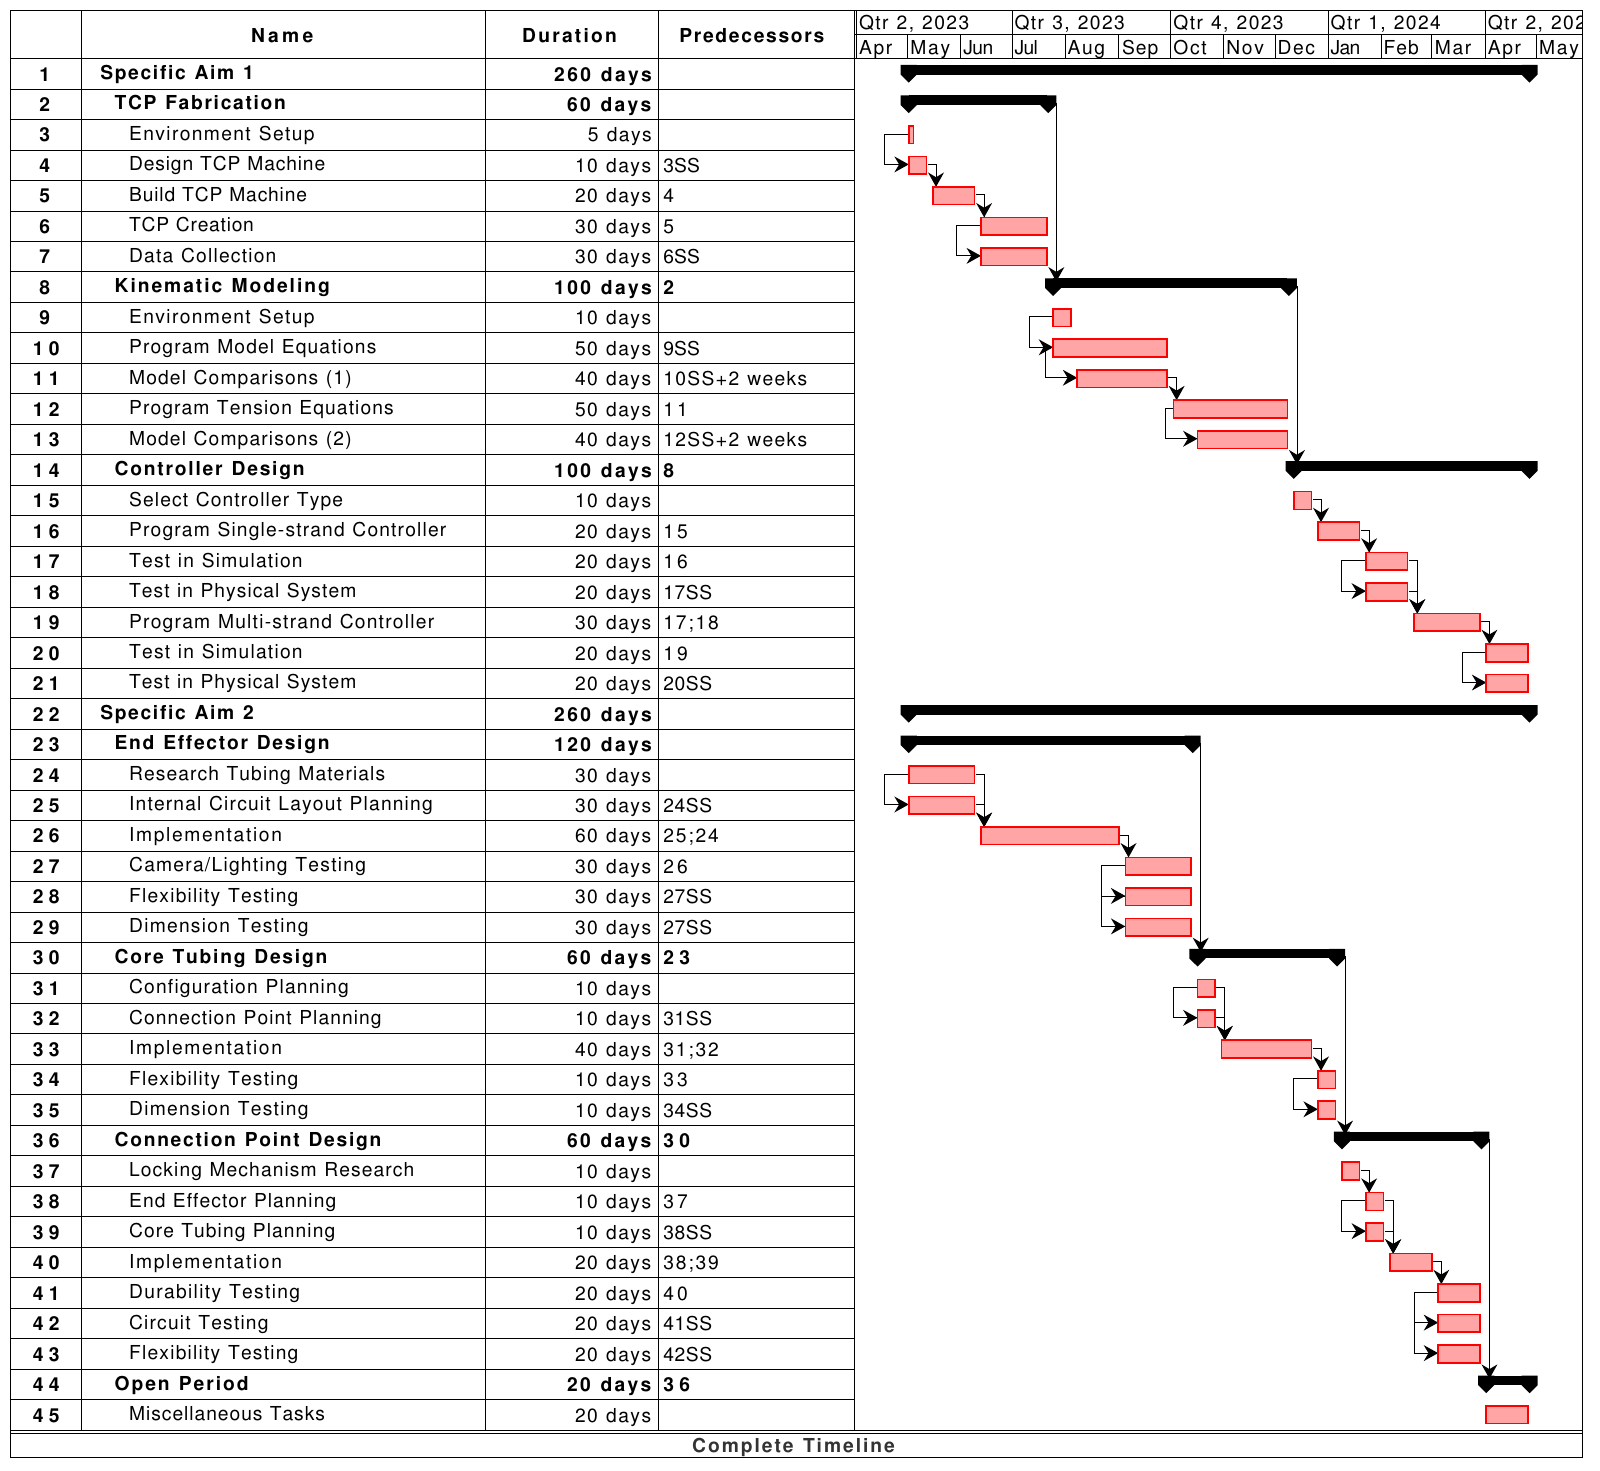
\includegraphics[scale=0.58]{full_timeline}
		\caption{Full AEI Project Timeline}
		\label{fig:full_timeline}
	\end{figure}

	\subsection{Aim 1: TCP Fabrication, Modeling, and Control}
	\label{subsect:aim1}
	
		Because of the unique properties of the actuation material, and for the purpose of data collection, the TCP material will be made in house. In the past, the material was created using a manually spun hand drill and imprecise counter-weight setup. With the intent of consistent recreation of the necessary string, the setup will be automated and configurable electronically. This step is very important to the overall performance of the project as consistency in the TCP material will be the difference between project success and project failure.
	
		Once the desired fabrication setup is complete, the arguably most difficult potion of the design process will begin. Here, the researchers will build symbolic kinematic modeling equations such that the TCP end effector can be simulated and controlled using an optimal feedback controller. This will gurrantee minimal error in intended versus actual movement. The system will be tested using inputs from a manual joystick controller, as well as with a predetermined path in order to simulate the inputs of the artificial intelligence system before it is officially ready for implementation (Aim 3).
	
	\subsection{Aim 2: Design of End Effector and Core Tubing}
	\label{subsect:aim2}
	
		In parallel to the modeling process, another objective is to design and implement the end effector and core tubing components. Since the end effector is objectively the highest risk component of the device, it will be designed to be completely removable from the rest of the core tubing. This will allow for easy replacement steps to be taken in the event of a broken end effector. With electrical connections set at designated positions, and held in place via a magnet and small locking mechanism.	 This is also where the camera at the end of the end effector (similar to the fiber optic camera) will be introduced and connected.
	
		The remainder of the core tubing design is composed of an outer shell, electrical wiring to each of the four TCP, and electrical wiring to the camera. These components will be developed separately from the end effector with the exception of the connection point, and will be light weight, with the objective of minimizing the diameter of the final tube, this step is not seen as a primary obstacle. Note that the outer tubing of both portions of the continuum component must be compatible with the human anatomy.
	
	\subsection{Aim 3: Integration Between Neural Network and Controller}
	\label{subsect:aim3}
	
		In the fall of the 2021-2022 academic year the original capstone team, composed of mechanical and biomedical engineering students, and based out of the Biomedical Engineering Department, created a separate project for the creation of a neural network which can identify the human airway anatomy. The intent was to develop software which would eventually guide the continuum robot by identifying anatomical features in the mouth of a patient. This project was largely successful due to the cooperation of the Computer Science and Engineering (CSE) Department, and the software created is ready for implementation with a finished prototype.
	
		Aim 3 of this project is to merge a final product with the artificial intelligence system created by the CSE team in the spring of 2022. This will consist of training a larger sample size of data, checking data conversions between the network and the main controller, and selecting a set of parameters which will be most useful in guiding the robot to the proper location.
